\documentclass[12pt,a4paper]{article}
\usepackage{times}
\usepackage{durhampaper}
\usepackage{harvard}


% ---------------------------------
% ---- PACKAGES -------------------
    % package to add wrapfigure
    \usepackage{wrapfig}
    % packages to add images
    \usepackage{graphicx}
    % packages for pseudocode and algorithms
    \usepackage{amsmath}
    \usepackage{algorithm}
    \usepackage[noend]{algpseudocode}
    \makeatletter
    \def\BState{\State\hskip-\ALG@thistlm}
    \makeatother
    % packages to generate neural network graph
    \usepackage{tikz}
    \usetikzlibrary{matrix,chains,positioning,decorations.pathreplacing,arrows}
    % package to add graphs
    \usepackage{pgfplots}
    % stuff for checkerboard
    \usetikzlibrary{matrix.skeleton}
    \tikzstyle{ball} = [circle, shading=ball, minimum size=1cm]
    \newcommand{\bl}{\node [ball, ball color=black!80!white, draw=black!65!white, thin]{};}
    \newcommand{\wh}{\node [ball, ball color=white] {};}
    \pgfplotsset{compat=1.15}
% ---- END PACKAGES ---------------
% ---------------------------------

    \citationmode{abbr}
    \bibliographystyle{agsm}
    % Titular Information
    \title{A Neuroevolutionary Approach to Draughts Playing Agents}
    \author{}
    \student{T. P. Nguyen}
    \supervisor{S. Dantchev}
    \degree{BSc Computer Science}
    \date{}

    % Start the Document
    % Note that the whole report, including the references, should not be longer than 20 pages in length.  The system will not accept any report longer than 20 pages.  It should be noted that not all the details of the work carried out in the project can be represented in 20 pages.  It is therefore vital that the Project Log book be kept up to date as this will be used as supplementary material when the project paper is marked.  There should be between 10 and 20 referenced papers---references to Web based pages should be less than 10\%.
    \begin{document}
    \maketitle
    % Doneish (WAIT FOR CONCLUSION)


\begin{abstract}
    % These instructions give you guidelines for preparing the final paper.  DO NOT change any settings, such as margins and font sizes.  Just use this as a template and modify the contents into your final paper.  Do not cite references in the abstract.

    % The abstract must be a Structured Abstract with the headings {\bf Context/Background}, {\bf Aims}, {\bf Method}, {\bf Results}, and {\bf Conclusions}.  This section should not be longer than half of a page, and having no more than one or two sentences under each heading is advised.

    {\bf Background}

    Presently, competitive Draughts AI players are currently designed to play at a fixed ability. While it has produced very competitive and intelligent players, they require some human intervention to improve their performance. 
    This is mostly due to their dependency on pre-defined move databases. Optimal moves are pre-calculated, and recalled when necessary. Through neuroevolution, this issue could possibly be solved by creating a player that can grow in ability over time, by learning to play itself.
    
    {\bf Aims}

    The purpose of this project is to explore an neuroevolutionary approach to tackle the game of English Draughts. First, we study previous historical successes in the field, and look at the components that helped build their systems. Then, we look at how they can be adapted to suit the objective at hand. The project will establish whether neuroevolution can be considered as a viable approach to the problem.

    {\bf Method}

    % The initial population consists of randomly generated AI players, which will play each other to determine the best player out of the population. The performance of championing AI players at every generation of the genetic algorithm are measured against previous champions. Appropriate algorithms are implemented to determine the overall development of the system's ability to play Draughts.
    The method starts with designing a feed-forward neural network that takes as input, the state of a checkerboard, and outputs an evaluation of the players advantage. This is then used in a algorithm that evaluates future moves to predict the best move at a given position. This, alongside a set of weights for the neural network, creates a player that can evaluate potential moves. Finally, the player is then used on an existing Draughts framework that will provide the player with the ability to play Draughts. Genetic algorithms are used to adjust the weights of the neural network, with the intention of making the system learn to evaluate checkerboards more precisely.
    
    {\bf Results}

    Overall, the neuroevolutionary approach ahs shown to learn and improve over time. The net learning rate was positive. However, the wide scope of the adjustments afforded may have impacted the learning rate and has shown to be volatile at some situations. The use of crossovers may dramatically influence the quality of the learning.

    {\bf Conclusion}

    Under the premise that the fitness function that is well defined, neuroevolution can be considered as an option to create a draughts playing AI. The robustness of the system is quite volatile, and is best paired with mutation and crossover methods that are not heavily reliant on entropy.

\end{abstract}
% Done
\begin{keywords}
    Artificial Intelligence, Machine Learning, Neural Networks, Neuroevolution, Genetic Algorithms, Draughts, Checkers, Crossover, Monte Carlo Tree Search
\end{keywords}
% DONE
\section{Introduction}
    % This section briefly introduces the general project background, the research question you are addressing, and the project objectives.  It should be between 2 to 3 pages in length.  Do not change the font sizes or line spacing in order to put in more text.
    The intention of this project is to explore the effectiveness of genetic algorithms to improve the neurons of a neural network. Neural networks can be used to evaluate the performance of two players in a zero-sum game of Draughts. We attempt to manipulate the neurons through the use of genetic algorithms to increase the accuracy of the evaluation. This would potentially allow us to create an effective Draughts playing agent that, when provided with the option to consider a set of moves, would have the ability to play and learn without human input.

    \subsection{Draughts}

    English Draughts (also Checkers) is a popular 2-player board-game played on an 8x8 chess board. Players choose a colour and begin with 12 pawns each of their respective colours, and they are placed on the dark-coloured squares of the board. Beginning with the black pawns, each player takes a turn to move a pawn diagonally in one square. In the event that a pawn reaches the opposite side of the board from where the piece originated, it is promoted to a king. Kings have the ability to traverse backwards in the same diagonal motion as pawns. Assuming that there is space upon landing, A piece (pawn or king) also has the option to capture their opponents piece by moving two consecutive diagonal squares, where the opponents piece is situated immediately opposing the players piece. Pieces can be captured consecutively in a single turn if the moves afford the scenario. A player wins by capturing all of their opponents pieces. A player loses by having all of their pieces captured. A draw occurs when both players agree to draw after a three-fold repetition (where both players take three moves to simulate the same position), or a player has pieces on the board but cannot move any of them. A draw can be forced when both players fail to capture a piece after a set amount of moves.

    \subsection{Neural Networks}

    Neural Networks are non-linear statistical data-modelling tools, linking inputs and outputs adaptively in a learning process similar to how the human brain operates. Networks consist of units, described as neurons, and are joined by a set of rules and weights. The units are defined with characteristics, and appear in layers. The first layer is defined as the input layer, and the last layer being the output. Layers between the two aforementioned are described as hidden layers. Data is analysed through their propagation through the layers of neurons, where each neuron influences the content of the data as they pass through. Learning takes place in the form of the manipulation of the weights connecting the units in the layers. This allows it to model complex relationships between inputs and output, and it can also find patterns in the data. 

 	\subsection{Genetic Algorithms}

    As subset of evolutionary algorithms in general, Genetic algorithms (GAs) are a group of search techniques used to find exact or approximate solutions to optimisation and search problems. The methodology is inspired by Charles Darwin's evolutionism theory; individuals are created by the crossover of the genetic information (genome) of their parents. Genomes are metaphors of genetic information; it typically refers to a data structure, most commonly an 1D array. Genetic Algorithms generally consist of a population of agents, a tournament selection process, algorithmic crossover mechanisms against the genomes of the agents, and the introduction of probabilistic mutation on genomes. The use of evolutionary algorithms to train neural networks is described as a type of machine learning called Neuroevolution.

    \subsection{Aims}

    % Research Question
    Whilst the use of evolutionary algorithms and neural networks have been explored to create draughts players, my intention is to explore the effectiveness of genetic algorithms and neural networks. The intention is to determine the possibility of developing a performing draughts playing agent by the use of Neuroevolution.

    \subsubsection{Minimum Objective}
        % The minimum objective of this project was to design and build a programme that would display a polygonal mesh of triangles, with help of a mesh data structure. The basic mesh data structure would have to enable future features that the next objectives would require.
        The minimum objective is to implement a feed-forward neural network, alongside a Draughts game interface for the network to evaluate on. This will need to pair with a decision making algorithm that determines the move to choose at a given state of the game. Finally, a simple genetic algorithm would also need to be implemented that interacts with the neural network.

    \subsubsection{Intermediate Objective}
        % The intermediate objective of this project was to create and incorporate the algorithms for the calculation of triangle surface normals, vertex normals and gradient (following our definition) in the initial programme, and enable visualisation of the “interesting” gradient changes and vertex normals on the mesh displayed by the programme.
        The intermediate objective involves the implementation of an interface to play against the trained result, and to create a monte-carlo decision making algorithm, which would be used by the agents to evaluate better decisions. Also, as the genetic algorithm includes a tournament mechanism which will play many games simultaneously, this will need to be implemented to run in parallel.
        
    \subsubsection{Advanced Objective}
        % The advanced objective of this project was to evaluate the speed of the algorithms and compare it to the time complexity that we obtained from theoretical analysis of the algorithms. The final sections of this paper will show the results acquired and the analysis and evaluation of the work we carried out. 
        The advanced objective consists of producing a system that indicates that it is learning over time. The later sections of this paper evaluates the quality of the learning rate and other results. 
    
    To template the document, the remaining sections of the paper discusses related and relevant work, the proposed solution, results and an evaluation of the project. Tha paper is then wrapped up with a conclusionary statement, discussing the implications of the project and potential future work.

% TODO
\section{Related Work}
    % This section presents a survey of existing work on the problems that this project addresses. it should be between 2 to 4 pages in length.  The rest of this section shows the formats of subsections as well as some general formatting information for tables, figures, references and equations.

    % Intro
        Although Draughts is a perfect information game, it has been historically used as a testing ground for artificial intelligence and computional performance since the early introduction of computers. This is due to the relatively vast search space, making it difficult to brute-force, until recently. Schaeffer proposed a method to solve the game \cite{schaeffer_solving_1996}, and with the perpetual improvement of computational capabilities, eventually followed on to prove that the game can be \emph{weakly-solved}. \cite{schaeffer_checkers_2007}. Weakly-solvable is defined such that ``the game-theoretic value for the initial position has been determined, and that a strategy exists for achieving the game-theoretic value from the opening position.'' \cite{allis_searching_1994} However, the premise of this paper is not necessarily to solve the game itself, but to rather see whether neuroevolution is a method that produce an agent that can play well.

        Research in artificial intelligence alone has been active since, targeting games with a higher move space, notably Chess and, more recently, Go. This section will summarise specific and notable techniques relevant to the discussion of the task at hand.

    % DONE
    \subsection{Arthur Samuel}
        In 1959, An early design of machine learning to play Draughts was devised by Arthur Samuel\cite{samuel_studies_1959}. His algorithm is based on the perpetual improvement of heuristics he devised, which act as an evaluator for a given state of the checkerboard. The evaluation function is calculated using the linear combination of his heuristics, which included various parameters of relevancy of the game. Some of these heuristics include the number of pawns and  number of pawns positioned along the central diagonal. His evolutionary strategy consisted of agents, each of which have different coefficent values for the heuristics (which are initiallised to have random values), and new agents are formed via the manipulation of its successor's coefficents with subtle mutations.
        
        % The weights were then trained by the algorithm playing itself in a form of genetic programming. 
        
        A later investigation by a checkers magazine evaluated Samuel's player to below Class B \cite{schaeffer_one_1997,fogel_evolving_2000} where Class B being categorised with an ELO range of [1600-1799]. However, the work described was naturally also dependent on a set of heuristics Samuel devised. This could handicap the agent's ability to play, as they are constrained on the quality of Samuel's heuristics. 

    % DONE
    \subsection{Blondie24}
        The idea of evolving neural networks to evaluate the game of Draughts is based on the success Chellapilla and Fogel had in evolving their own draughts playing neural networks. Their method used Samuel's system as a foundation and modified the evaluation method, using feed-forward neural networks instead of a distinct  linear combination. Their resulting player, Blondie24, was then taught to play without priori knowledge, in a similar vein to Samuel's system, but played at a higher level of competency. \cite{chellapilla_evolving_1999}

        Blondie24 uses an evolutionary algorithm, using fifteen agents $i=1,\dots,15$, each of which consisted of two properties. The first property were weights of the neural network (which are initially random), with the second property being a self-adaptive parameter vector, $\tau_i$, which determined how random the mutations are when the agent $i$ evolved. 

        \begin{figure}[ht!]
            \centering
            \begin{equation}
            \tau_i(j) = \tau_i(j) \cdot e^{\mu}
            \end{equation}
            \caption{The mutation formula in Blondie24, where $j=1,...,N_w$ represents individual weight of the neural network $w$, and $\mu$ representing a random decimal in the range of $[0-1]$. \label{blondieMutation}}
        \end{figure}
        
        In each generation, every agent plays each other in a round robin style tournament. Every agent plays an equal amount of games, and successors are chosen based on their performance in the tournament. The best agents are chosen to mutate themselves to produce new agents. Mutation is performed using the formula in Figure \ref{blondieMutation}.    

        However, crossover mechanisms were not considered (and is thus cannot be classified as using genetic algorithms). Blondie24's neural network structure consists of a $\left\{ 32,40,10,1 \right\}$ set, such that the input layer consisted of 32 nodes, and a single output node. The output node consists of a classifier value that has a range of [-1, 1], representing a particular advantage for a given side of the board. One fallback that can be seen with this particular method is that spatial awareness is not considered as it takes an immediate input of the positions on the board. This makes it inherently more difficult for the neural network to generate heuristics based on spatial awareness. Relative distance between pieces are not encapsulated in a method that can be immediately interpreted by the neural network.

        Blondie24's decision making algorithm primarily revolved around a mini-max algorithm with a ply cap. This algorithm takes as input the present state of the checkerboard, and returns the best move to choose. The mini-max algorithm is described using the following instructions:
        
        \begin{enumerate}
            \item Each node represents a state of a checkerboard. Child nodes represent a future state of the checkerboard, given a move. Child nodes can only be produced from the parent node; i.e. a move from a parent node will produce a child node.
            \item Child nodes are expanded until some depth is reached. From here, an evaluation function is used to calculate the value of the leaf nodes at this depth. This evaluation function produces a value that indicates a players advantage in a given state.
            \item The best potential position for a given player can be deduced from the nodes at this stage, which is quantified with a value.
            \item The best value propagates upwards until it reaches to a child of the root node. This represents an agent's current state of the game.
        \end{enumerate}

        The use of alpha-beta pruning would help to ignore evaluating disadvantageous moves, reducing the number of neural network evaluations. Once the possible moves have been considered, the best child node is chosen, representing the best move at a given position.
    
        There are inherent trade-offs to this decision algorithm, especially with utilising higher ply counts; asymptotic complexity of mini-max is exponential; it being $O(x^y)$ for $x$ being the branching factor, and $y$ being depth. The branching factor consists of the moves from each agent in a given game. This exponential growth is the achilles heel to the mini-max approach. 

        We do not wish to repeat this work, but it is important to understand that we wish to abstract and modularise parts of the best features of this system to modify and extend them to the solution described in the paper.

    \subsection{Post Blondie24}

        Blondie24 was influential in the field of neuroevolution during its time, leading to various studies on the theory behind its success. A notorious example is the series of publications by Al-Khateeb and Kendall, where they explore in detail the different features that comprise Blondie24. One of their studies concerning the effects of the the Look-ahead Depth (or ply) conlcuded that having a higher ply-depth unsurprisingly increases the overall performace of the player, and that agents trained at a higher ply performs significantly worse when playing at a lower ply. More importantly, the results in the paper suggest that a 4ply depth produces the best value function to start with during the learning phase, and increasing the ply depth for evaluations. \cite{al-khateeb_effect_2012} Their study in the influence of tournaments in Blondie24 concluded that the league structure seemed more appropiate to use as opposed to the round robin tournament. \cite{al-khateeb_introducing_2009} This is however more difficult to parallelise, which may be a largely contributing factor during the implementation of the system.
        
        % Alternative contemporary machine learning techniques have been exercised against Draughts. Franken et al. (2003) used draughtsboards as an evaluator for their rendition of an AI through Particle Swarm Optimisations.[14] 
        Within research in the game of Draughts alone, A research by Toledo-Marin et al. looked at studies on attacking strategies using Draughts as a reference (which however can be applied to any other zero-sum game), where they mathematically prove that for an offensive player, maximising the offensive improves their probability to win.\cite{toledo-marin_is_2016} This could be considered to guide the system to lean towards attacking moves, which could potentially accelerate the learning rate of the system.

        % Stanford's SVM method of improving Blondie
        % Cobbe, et al. improves Blondie24 by using an evaluation function that consists of Support Vector Machines, which achieves locally optimal performance in approximately a third as many generations than its typical evolution. \cite{cobbe_accelerating_nodate} 
        
    % TODO: fix writeup of everything, talk about monte-carlo
    % \subsection{Neural Networks}
    %     % need to mention regular gradient based learning
    %     Lai's Giraffe \cite{lai_giraffe:_2015} program used a deep reinforcement learning technique to play Chess to an advanced level in a relatively quick time-period. Giraffe's decision function involved using Temporal Difference Learning (TD-Leaf), an improvement on MiniMax, by Baxter et al. \cite{baxter_tdleaflambda_1999} However, Giraffe has been trained on previously played games from grandmaster tournaments as a reference, and was not entirely self-taught.
        % Lai then moved on to join DeepMind, 

        % talk about monte-carlo

    % TODO: fix writeup of everything
    \subsection{Return of Genetic Algorithms}

        Since then, there has been a non-trivial number of published papers describing the promising utility of genetic algorithms and neural networks in general. Genetic algorithms have been shown to evolve weights for a convolutional neural network in a classification task better than back-propagation, in nearly all situations, other than when the number of generations generated for neural networks are small. \cite{perez_apply_nodate} Another research showed its ability to compute optimal structures for deep neural networks, using an image recognition dataset as the benchmark for competitiveness against the networks. \cite{xie_genetic_2017}
        
        % Kusiak et al. (2007) have devised the use of pure genetic algorithms as the premise to evaluate the board. [16] they describe the use of 25 heuristics that, when used in unison, can determine the evaluation of a given board. They continue to go further on and specify that various combinations of heuristics, when used in different stages of the game, prove to be the most promising of outcomes.

        % Uber's revival of genetic algorithms and safe mutations
        However, one recent paper by Clune et al. on behalf of Uber Labs returned to the use of genetic algorithms as a basis to train especially deep convolutional networks with success. \cite{such_deep_2017} Their neuroevolutionary system was used to play popular Atari games on the OpenAI framework, and was found to perform as well as other contemporary evolution strategies and reinforcement learning algorithms. 

        The success of the program was based on their system's ability to perform safe mutations, a technique that revolves around measuring the sensitivity of the network to changes with some of the weights. \cite{lehman_safe_2017} This afforded the system to evolve deep neural networks (In this particular case, containing over 100 layers and over four million weights and biases,) in a manner that allowed random but safe and exploratory s.pdf. Their safe mutation exploits the knowledge of the neural network structure, by retaining sampled experiences of the network (inputs that feed into the network and its outputs). This allows the weights to be manipulated by comparing its significance with the output, by comparing it with the sampled experiences. 

        However, they also do not consider the use of crossover techniques in their paper. It is discussed that it would very well be possible to produce a safe crossover method that can exploit structures of a neural network, inspired by their research produced on safe mutations.

        Unfortunately, it is unrealistic to apply the same techniques described in their paper into the proposed system. The machine used as the base (consisting of hundreds to thousands of cores) is of a magnitude greater than what is available for the task at hand, but a more simplistic and adapted model can be produced using similar ideas. 
        
        A popular trend between the aforementioned papers is that there is a trend of absence of the use of crossover algoirithms. One paper describes the use of different crossover algorithms on neural networks having no clear advantage over each other, in comparison to a uniform crossover (uniform crossovers are also commonly defined as the textbook crossover) which disrupted the overall performance of the neural networks. This could be due to building blocks being disrupted as chunks of the sequential weights are swapped out of each other. \cite{emmanouilidis_comparison_2000} It is important to consider this when devising a crossover method, such that the effect it has on the neural network should be subtle enough that it should pose similar results to the network prior to crossovers.

% TODO: Write up everything..
\section{Solution}

    % This section presents the solutions to the problems in detail.  The design and implementation details should all be placed in this section.  You may create a number of subsections, each focussing on one issue.  

    % This section should be between 4 to 7 pages in length.
        
    This section describes the implementation process of the system. Implementing the checkerboard interface is not included in the discussion as it is not one of our objectives. However, the sections below are considered under the premise that the interface is built prior. The system was implemented using Python 3.6 and NumPy.

    \subsection{Evaluation Function}
        % Neural Net figure
        \begin{figure}[ht!]
            \centering
            \caption{The chosen neural network model. The preprocessed values of the checkerboard are used as input. An output is produced after propagation that ranges from [-1,1]. \label{nnmodel}}
            \vspace{10pt}
            \tikzset{%
                every neuron/.style={
                    circle,
                    draw,
                    minimum size=0.9cm
                    },
                neuron missing/.style={
                    draw=none, 
                    scale=4,
                    text height=0.333cm,
                    execute at begin node=\color{black}$\vdots$
                },
            }

            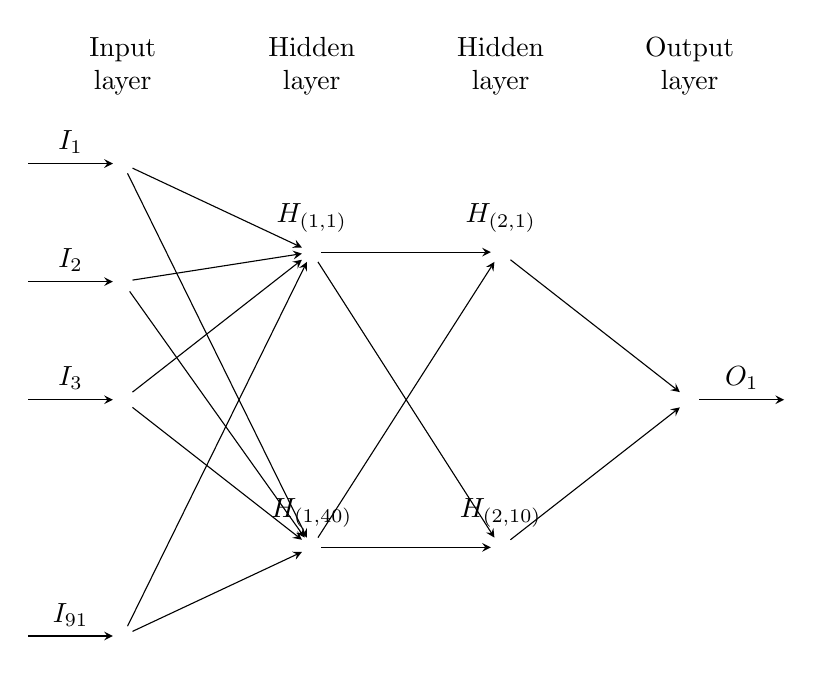
\begin{tikzpicture}[x=1.2cm, y=1.5cm, >=stealth]

            % draw nodes
                % % input values
                % \foreach \m/\l [count=\y] in {1,2,3,missing,4}
                % 	\node [every neuron/.try, neuron \m/.try] (input-\m) at (-0.5,2.5-\y) {};

                % input layer
                \foreach \m/\l [count=\y] in {1,2,3,missing,4}
                \node [every neuron/.try, neuron \m/.try] (input-\m) at (0,2.5-\y) {};
                
                % layer 1
                \foreach \m [count=\y] in {1,missing,2}
                \node [every neuron/.try, neuron \m/.try ] (hidden1-\m) at (2,2-\y*1.25) {};

                % layer 2
                \foreach \m [count=\y] in {1,missing,2}
                \node [every neuron/.try, neuron \m/.try ] (hidden2-\m) at (4,2-\y*1.25) {};

                % output layer
                \foreach \m [count=\y] in {1}
                \node [every neuron/.try, neuron \m/.try ] (output-\m) at (6,0.5-\y) {};

            % input layer
            \foreach \l [count=\i] in {1,2,3,91}
                \draw [<-] (input-\i) -- ++(-1,0)
                node [above, midway] {$I_{\l}$};

            % hidden 1
            \foreach \l [count=\i] in {{(1,1)},{(1,40)}}
                \node [above] at (hidden1-\i.north) {$H_{\l}$};

            % hidden 2
            \foreach \l [count=\i] in {(2,1),(2,10)}
                \node [above] at (hidden2-\i.north) {$H_{\l}$};

            % output layer
            \foreach \l [count=\i] in {1}
                \draw [->] (output-\i) -- ++(1,0)
                node [above, midway] {$O_\l$};

            % lines from input to hidden 1
            \foreach \i in {1,...,4}
                \foreach \j in {1,...,2}
                    \draw [->] (input-\i) -- (hidden1-\j);
            
            % lines from hidden 1 to hidden 2
            \foreach \i in {1,...,2}
            \foreach \j in {1,...,2}
                \draw [->] (hidden1-\i) -- (hidden2-\j);

            % lines from hidden 2 to output
            \foreach \i in {1,...,2}
                \foreach \j in {1}
                    \draw [->] (hidden2-\i) -- (output-\j);

            % headings
            \foreach \l [count=\x from 0] in {Input, Hidden, Hidden, Output}
                \node [align=center, above] at (\x*2,2) {\l \\ layer};

            \end{tikzpicture}
            % \vspace{-25pt}
        \end{figure}
        
        % \begin{wrapfigure}{r}{0.37 \textwidth}
            %     % \begin{center}
            %     \fontsize{8}{11}
            %     % \vspace{-40pt}
            %     \centering
            %         \caption{The indexes of the 32 pieces of the input layer are the immediate values of the positions on the board. \label{boardarray}}
            %         \vspace{5pt}
            %         \begin{tikzpicture}
            %         \color{white}
            %         \matrix (m) [matrix of nodes, nodes in empty cells, label skeleton, nodes={minimum size = 0.4cm}] {
            %         & 31 &&30&&29&&28 \\
            %         27 &&26&&25&&24&&\\
            %         &23&&22&&21&&20\\   
            %             19&&18&&17&&16&&\\
            %         &15&&14&&13&&12\\
            %         11&&10&&9&&8&&\\
            %         &7&&6&&5&&4\\
            %         3&&2&&1&&0\\
            %         % \bl &     & \bl &     &     &     & \bl &     \\
            %         %     &     &     & \bl &     &     &     &     \\
            %         % \wh &     &     &     &     &     &     &     \\
            %         %     &     &     & \wh &     & \wh &     & \wh \\
            %         % \wh &     & \wh &     & \wh &     & \wh &     \\
            %         %     & \wh &     & \wh &     & \wh &     & \wh \\
            %         };
            %         \foreach \row in {1, ..., 8} {
            %         \foreach \col in {1, ..., 8} {
            %             \pgfmathparse{Mod(\row + \col, 2) ? "black" : "white"}
            %             \colorlet{squarebg}{\pgfmathresult}
            %             \fitandstyle[background]{(m-cell-\row-\col)}{fill = squarebg}
            %         }
            %         }
            %         \end{tikzpicture}
            %     % \end{center}
            %     \vspace{-20pt}
            % \end{wrapfigure}
            % % talk about how it works
            % % talk about the preprocessing
        
        A feed-forward multilayer perceptron neural network was used to evaluate the board. The network contained 4 layers; the input layer consists of 91 nodes, with the output node having 1. Hidden layers had 40 and 10 nodes respectively. Figure \ref{nnmodel} shows the network in the form of a diagram.

        The inputs of the network is a preprocessed 1D array of the checkerboard. Preprocessing the input starts with retrieving the positions of the pieces on the checkerboard in the form of an 1D array, and calculating all possible individual subsquares of the board. The subsquares kernel size range from a 3x3 to an 8x8 size. Figure \ref{subsquares} visualises the retrieval of the subsquares. With the kernels, the values of the pieces in the subsquare is summed up. A new array is formed, comprising of the sums of the different kernels that comprise the board. This new array (comprised of 91 entries) represents the preprocessed input, which is then fed to the neural network.

        To create values for the subsquares, the black pawns were weighed with a value of $v=1$, and white pawns as $-v$. It is commonly understood that a king is worth more than a pawn piece, but it is disputed about its precise value advantage. This could be decided by the system such that could can evolve to understand that a King is eventually worth more than the pawn. For the sake of simplicity however, a king's piece value was weighted at $1.5v$.

        \begin{figure}[!h]
            \centering
            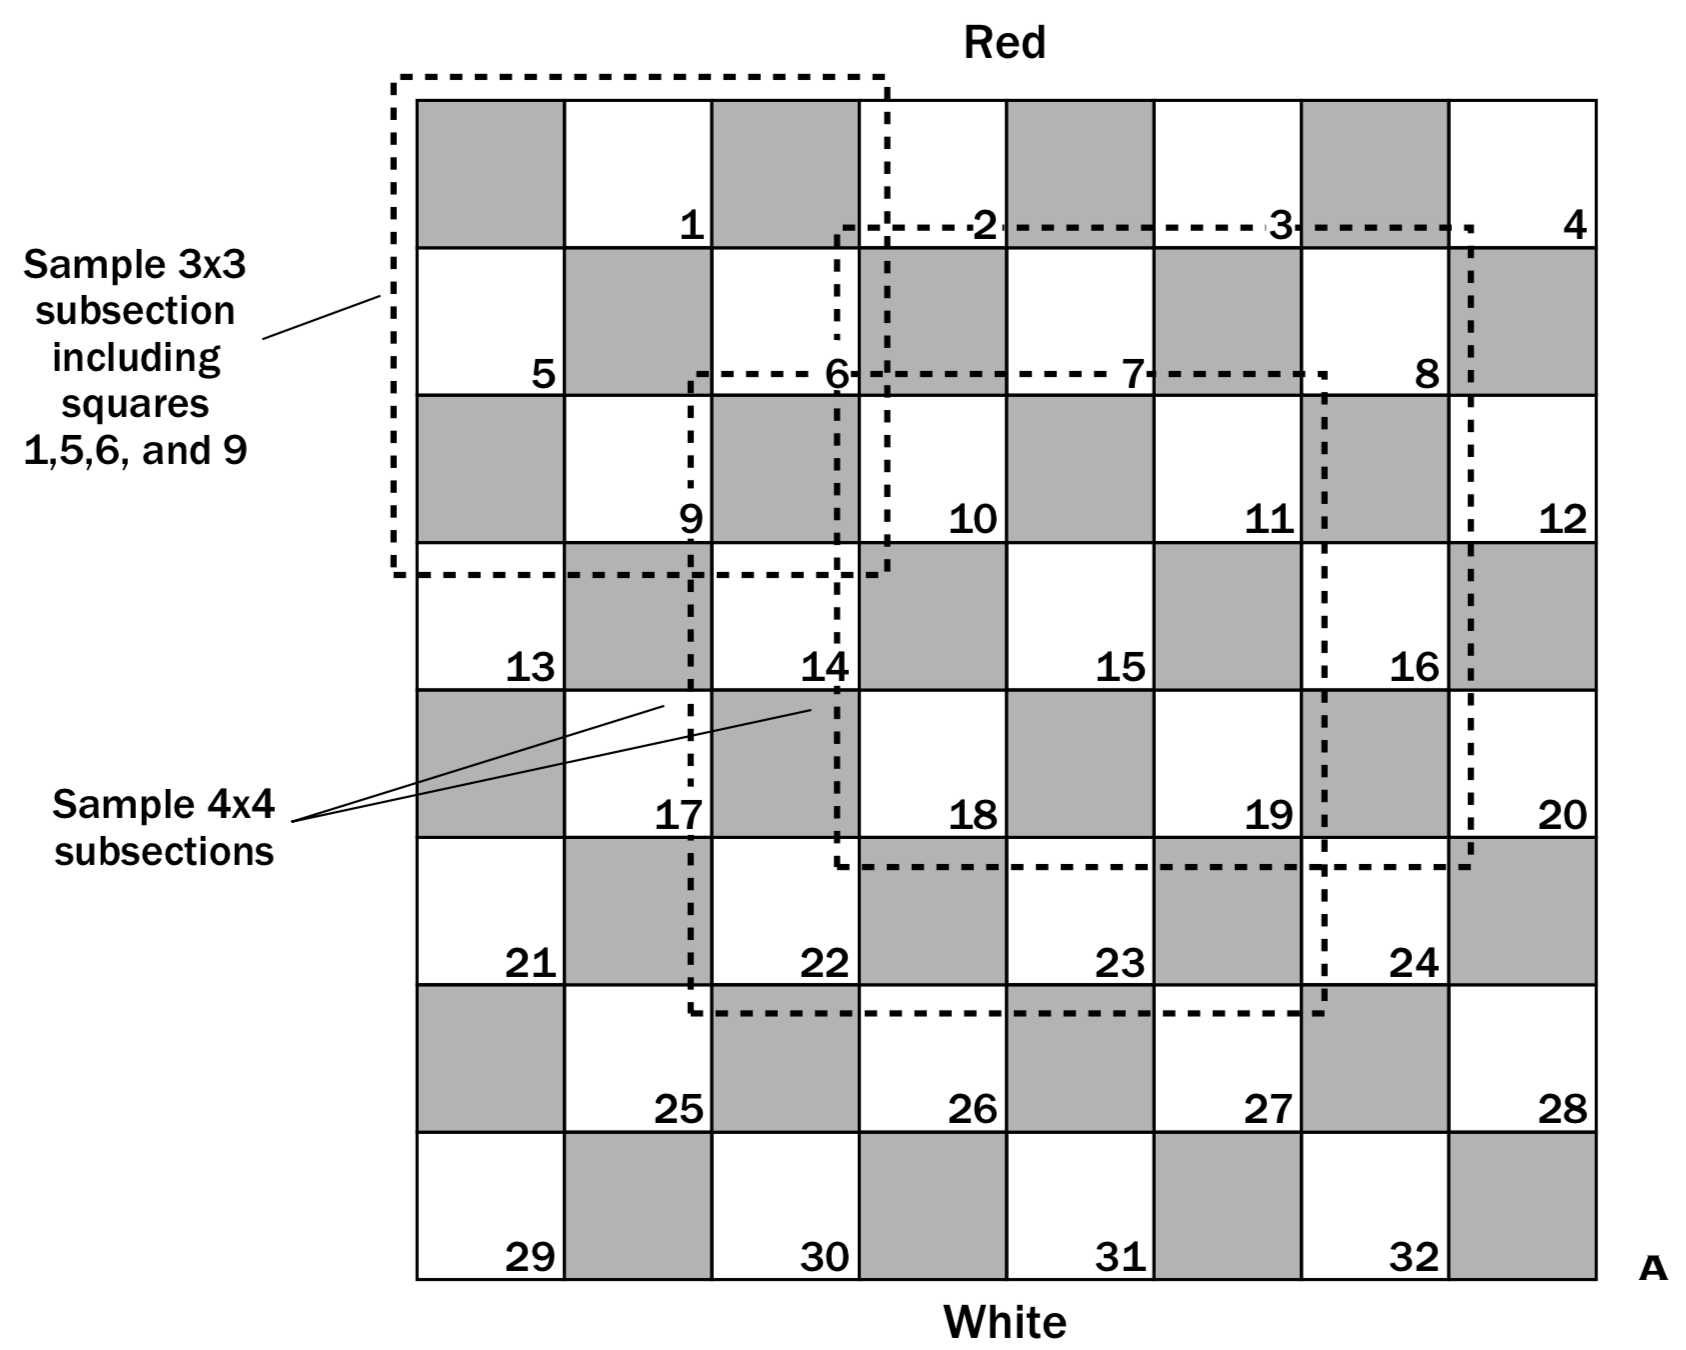
\includegraphics[width=90mm]{images/subsquares.png}
            \caption{A diagram visualising the processing of subsquares.\label{subsquares}}
        \end{figure}

        % Talk about the activation function
        Weights $w$ of a neuron are multiplied by their input value $I$, summed with their bias $B$, and are passed through an activation function $O = f((I* w) + B)$ to become an input for another neuron. Activation functions, when visualised, usually have a sigmoid curve, but may also take the form of other shapes. Common characteristics of activation functions include values to be monotonically increasing, continuous, differentiable and bounded.
        % how does it work?

        % Tanh Diagram
        \begin{wrapfigure}{r}{0.4\textwidth}
            \centering
            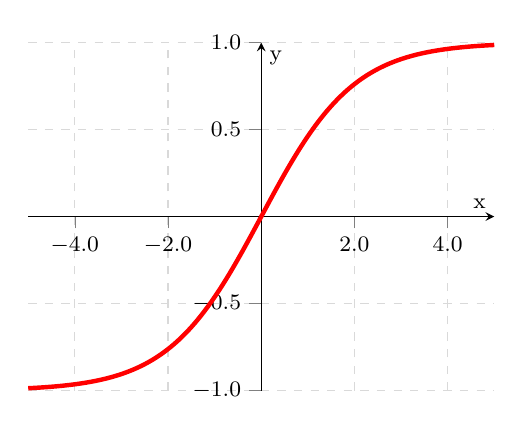
\begin{tikzpicture}
                \fontsize{8}{11}
                \begin{axis}[
                    legend pos=north west,
                    axis x line=middle,
                    axis y line=middle,
                    x tick label style={/pgf/number format/fixed,
                                        /pgf/number format/fixed zerofill,
                                        /pgf/number format/precision=1},
                    y tick label style={/pgf/number format/fixed,
                                        /pgf/number format/fixed zerofill,
                                        /pgf/number format/precision=1},
                    grid = major,
                    width=75mm,
                    height=6cm,
                    grid style={dashed, gray!30},
                    xmin=-5,     % start the diagram at this x-coordinate
                    xmax= 5,    % end   the diagram at this x-coordinate
                    ymin= -1,     % start the diagram at this y-coordinate
                    ymax= 1,   % end   the diagram at this y-coordinate
                    %axis background/.style={fill=white},
                    xlabel=x,
                    ylabel=y,
                    tick align=outside,
                    enlargelimits=false]
                % plot the stirling-formulae
                \addplot[domain=-5:5, red, ultra thick,samples=500] {2*(1/(1+e^-x))-1};
                % \addlegendentry{$f(x)=\frac{1}{1+e^{-5x}}$}
                \end{axis}
            \end{tikzpicture}
            \caption{Graph of tanh function $f(x)={\frac{2}{1+e^{-x}}- 1}$ (An example of an activation function with a sigmoid curve). \label{sigmoid}}
            \vspace{-10pt}
            \end{wrapfigure}

        Our choice for the activation function is tanh (a type of sigmoidal function), shown in figure \ref{sigmoid}. 
        % There exists inherent issues related to the properties of their derivatives, commonly known as the missing gradient problem. This is an issue  \cite{nair_rectified_2010}, described as the missing gradient problem. However, since this issue is related to the properties of a gradient based learning method and not through a stochastic learning method (of which genetic algorithms are), this is not a concern for the project. 
        The use of tanh facilitates the ability to simulate a zero sum formula (for a range of [-1 to 1]) due to its symmetric properties around the origin.
        
        Results are cached such that evaluations are saved such that they can be recalled immediately, in the event that the same input is evaluted. This has shown varying levels of time improvement dependent on the ply depth. As the ply increases, the size of the state space increases, and therefore the chances of recalling the same set of inputs decrease. The cache is also used for our safe mutations algorithm, described later on in Section \ref{coefficient_mutation}.

        The neural network was implemented manually using the NumPy library to allow direct access to the weights, allowing the genetic algorithm access to manipulate them.
    
    % DONE
    \subsection{Decision Making Algorithm}
        Initially, the decision making algorithm chosen is the same mini-max approach as in Blondie24, but is then progressed to a modified Monte-Carlo Tree Search (MCTS). A basic MCTS differs from mini-max where future moves are randomly played to the end of the game. It acts as a sampling of possible outcomes, and does not depend on an evaluation function at all. The random simulation of games are skewed such that more reasonable moves are chosen. A survey found that MCTS can dramatically outperform mini-max based search engines in games where evaluation functions are otherwise difficult to obtain \cite{browne_survey_2012}. In worst case situations, MCTS is also found to converge towards Mini-Max. MCTS is played in rounds that consist of four operations:

        \begin{itemize}
            \item Selection: A selection strategy is played recursively until some position is reached. 
            \item Play-Out: A simulated game is played. Again, a basic form of MCTS would play until an end-game is reached.
            \item Expansion: A node is added to the tree.
            \item Back-propagation: The result of the game is back-propagated in the tree of moves.
        \end{itemize}

        These rounds are repeated until a certain period of time is met or a certain number of rounds are computed. Once finished, a node is chosen based on its total probability of reaching an winning outcome.

        \begin{figure}[!h]
            \centering
            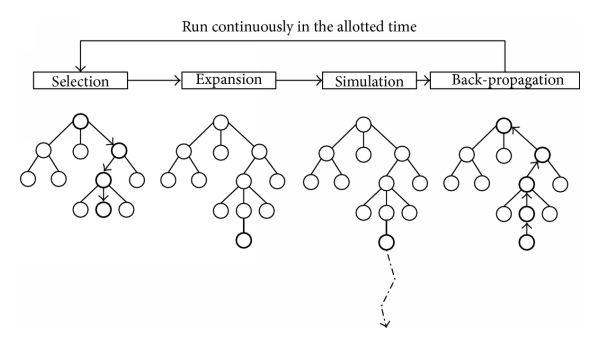
\includegraphics[width=100mm]{images/montecarlo.png}
            \caption{A diagram describing the MCTS process.}
        \end{figure}

        MCTS-EPT (or MCTS with early playout termination) modifies MCTS random play-out approach; Instead of allowing the random moves play to the end of the game, the number of moves traversed are capped and an evaluation function (which in our case is the neural network) is applied at that future state instead. \cite{lorentz_using_2016} The model has been adapted such that if the number of possible moves is less than 4, the ply depth is extended by the number of moves. This reduces the need to depend on random playouts of moves to the end, and ensures that the quality of the moves is contingent on the evaluation function. For our results, we use the ply depths 1,3 and 6 to determine the system is consistent. As opposed to using a time threshold, the number of MCTS rounds $r$ is based on the ply depth $p$, such that $r=300p$. This allows the system to process moves in a manner that the performance of the system is hardware-independent, as faster machines could process more rounds in a fixed set of time.

        % talk about the fact that this is a probabilistic strategy

        % The minimax algorithm would be retained to evaluate the performance differences between the two decision making algorithms.

    \subsection{Genetic Algorithms}
        % talk about generation of population
        % talk about tournmanent
        % talk about 
        The genetic algorithm is the premise of the system's learning strategy. GA's are used to train the neural network. We discuss the various algorithms that form the collection of GA strategies below. For the system, a population size of 15 was chosen.

        \subsubsection{Population Generation} \label{population_generation}
            % Introduce what its for
            In genetic algorithms, the population serves as a base that allows agents in the pool to play each other. Every generation has its own population of agents, and the population size is consistent of the generations. The initial population consisted of randomly generated weights and biases of the neural network, with values from [-1,1]. 
            
            For a population size of 15, the next generation was created using the best five agents from the current generation (discussed in {\it{\ref{tournament_selection} Tournament Selection}}.) They would continue to play in the next generation; this strategy is described as elitism. The next eight players are generated through the use of crossover strategies (see {\it{\ref{crossover_strategy} Crossover Strategy}}). The weights of the $1^{st}$ and $2^{nd}$ place agents are used as input to the crossover strategy and will generate 4 offsprings. Two are reciprocal crossover representations from each other, and the other two being directly mutated from the parents themselves. Another four children will be created using the same strategy, with the 2nd and 3rd agent's weights. The remaining two will be direct mutations of the 4th and 5th place agents.

        \subsubsection{Tournament Selection} \label{tournament_selection}

            To sort the quality of the players in a population, a tournament selection process is deduced. This allows us to choose the best players who will continue to play in the next generation.

            Currently, each agent in the population would play 5 games as Black, against randomly selected opponents. Each game lasts a maximum of 100 moves from both players. If a winner is not deduced at this stage, a draw is called. Draws are also called when there is a three-fold move repetition from both players. A win is worth $2$ points, a draw being none and a loss being $-1$ points. Both the agent and its opponent receives a score from the game.
            Scores are tallied up at the end of the tournament. Players are sorted by the number of points they scored. The best players would have the highest number of points.
            
            All of the games are run 'embarrasingly parallel' through the use of Python's multiprocessing library. Whilst the league structure was found as the better approach \cite{al-khateeb_introducing_2009} it would increase the overall running time as the initialisation of some games are dependent on the outcomes of other games.
            
        \subsubsection{Coefficient Mutation} \label{coefficient_mutation}

            \begin{figure}
            \begin{equation}
                % \caption{The mutation formula. \label{mutation}}
                w_n = w_p + \frac{m}{\sqrt{2 * \sqrt{K} }}
            \end{equation}
            \caption{The mutation formula, where $w_p$ is the current weight, $K$ represents the number of weights and biases in the neural network, and $m$ representing a random floating point in the range of [-1,1].\label{mutation}}
            \end{figure}

            To create variation between agents and their offspring, statistical anomalies are made through the use of mutations. This is used as one of the learning mechanisms that help change the decision factors of the neural network. Weight and biases of an agent's neural network would increment by a random value that is created using the equation in Figure \ref{mutation}.

            Like the activation function,
            % (in \ref{sigmoid})
            the weights would have a soft maximum of [-1, 1]. This consequently meant that the mutation was not controlled, but rather dependent on the number of weights in the system; The more weights in the network implies a less significant mutation. Soft mutation \cite{lehman_safe_2017} is also used. We use a subset of historical neural network calculations as a premise to guide our mutation. The method is as follows:
             
             \begin{enumerate}
             \item With the current set of weights $w$, choose a subset of precalculated input and output tuples $\phi_{w} = (I, \lambda_{I,w})$ where $I$ represents the input values of the network, and $\lambda_{I,w}$ as the output.
             \item Generate a perbutation $y$ of the weights calculated using the formula in Figure \ref{mutation}. Use $y$ as a basis of a neural network. 
              \item Using the inputs $I$ in $\phi_{w}$, calculate a new set of input and output tuples $\phi_{y} = (I, \lambda_{I,y})$.
              \item Calculate the divergence $\delta = \lambda_{I,y} /\ \lambda_{I,w}.$ 
              \item Calculate the quality of $y$ based on the number of inequalities $\delta \geq 1$.
             \item Repeat parts 2-5 some $n$ times, keeping note of the the best $y$. 
             \end{enumerate}

            The intuition behind this is that if $\phi_{w}$ is a subset of moves that led to a winning game, then the manipulation of the weights is left open as long as it can replicate the performance of winning games.
            
        \subsubsection{Crossover Strategy} \label{crossover_strategy}

                
           \begin{figure}[!ht]
                \centering
                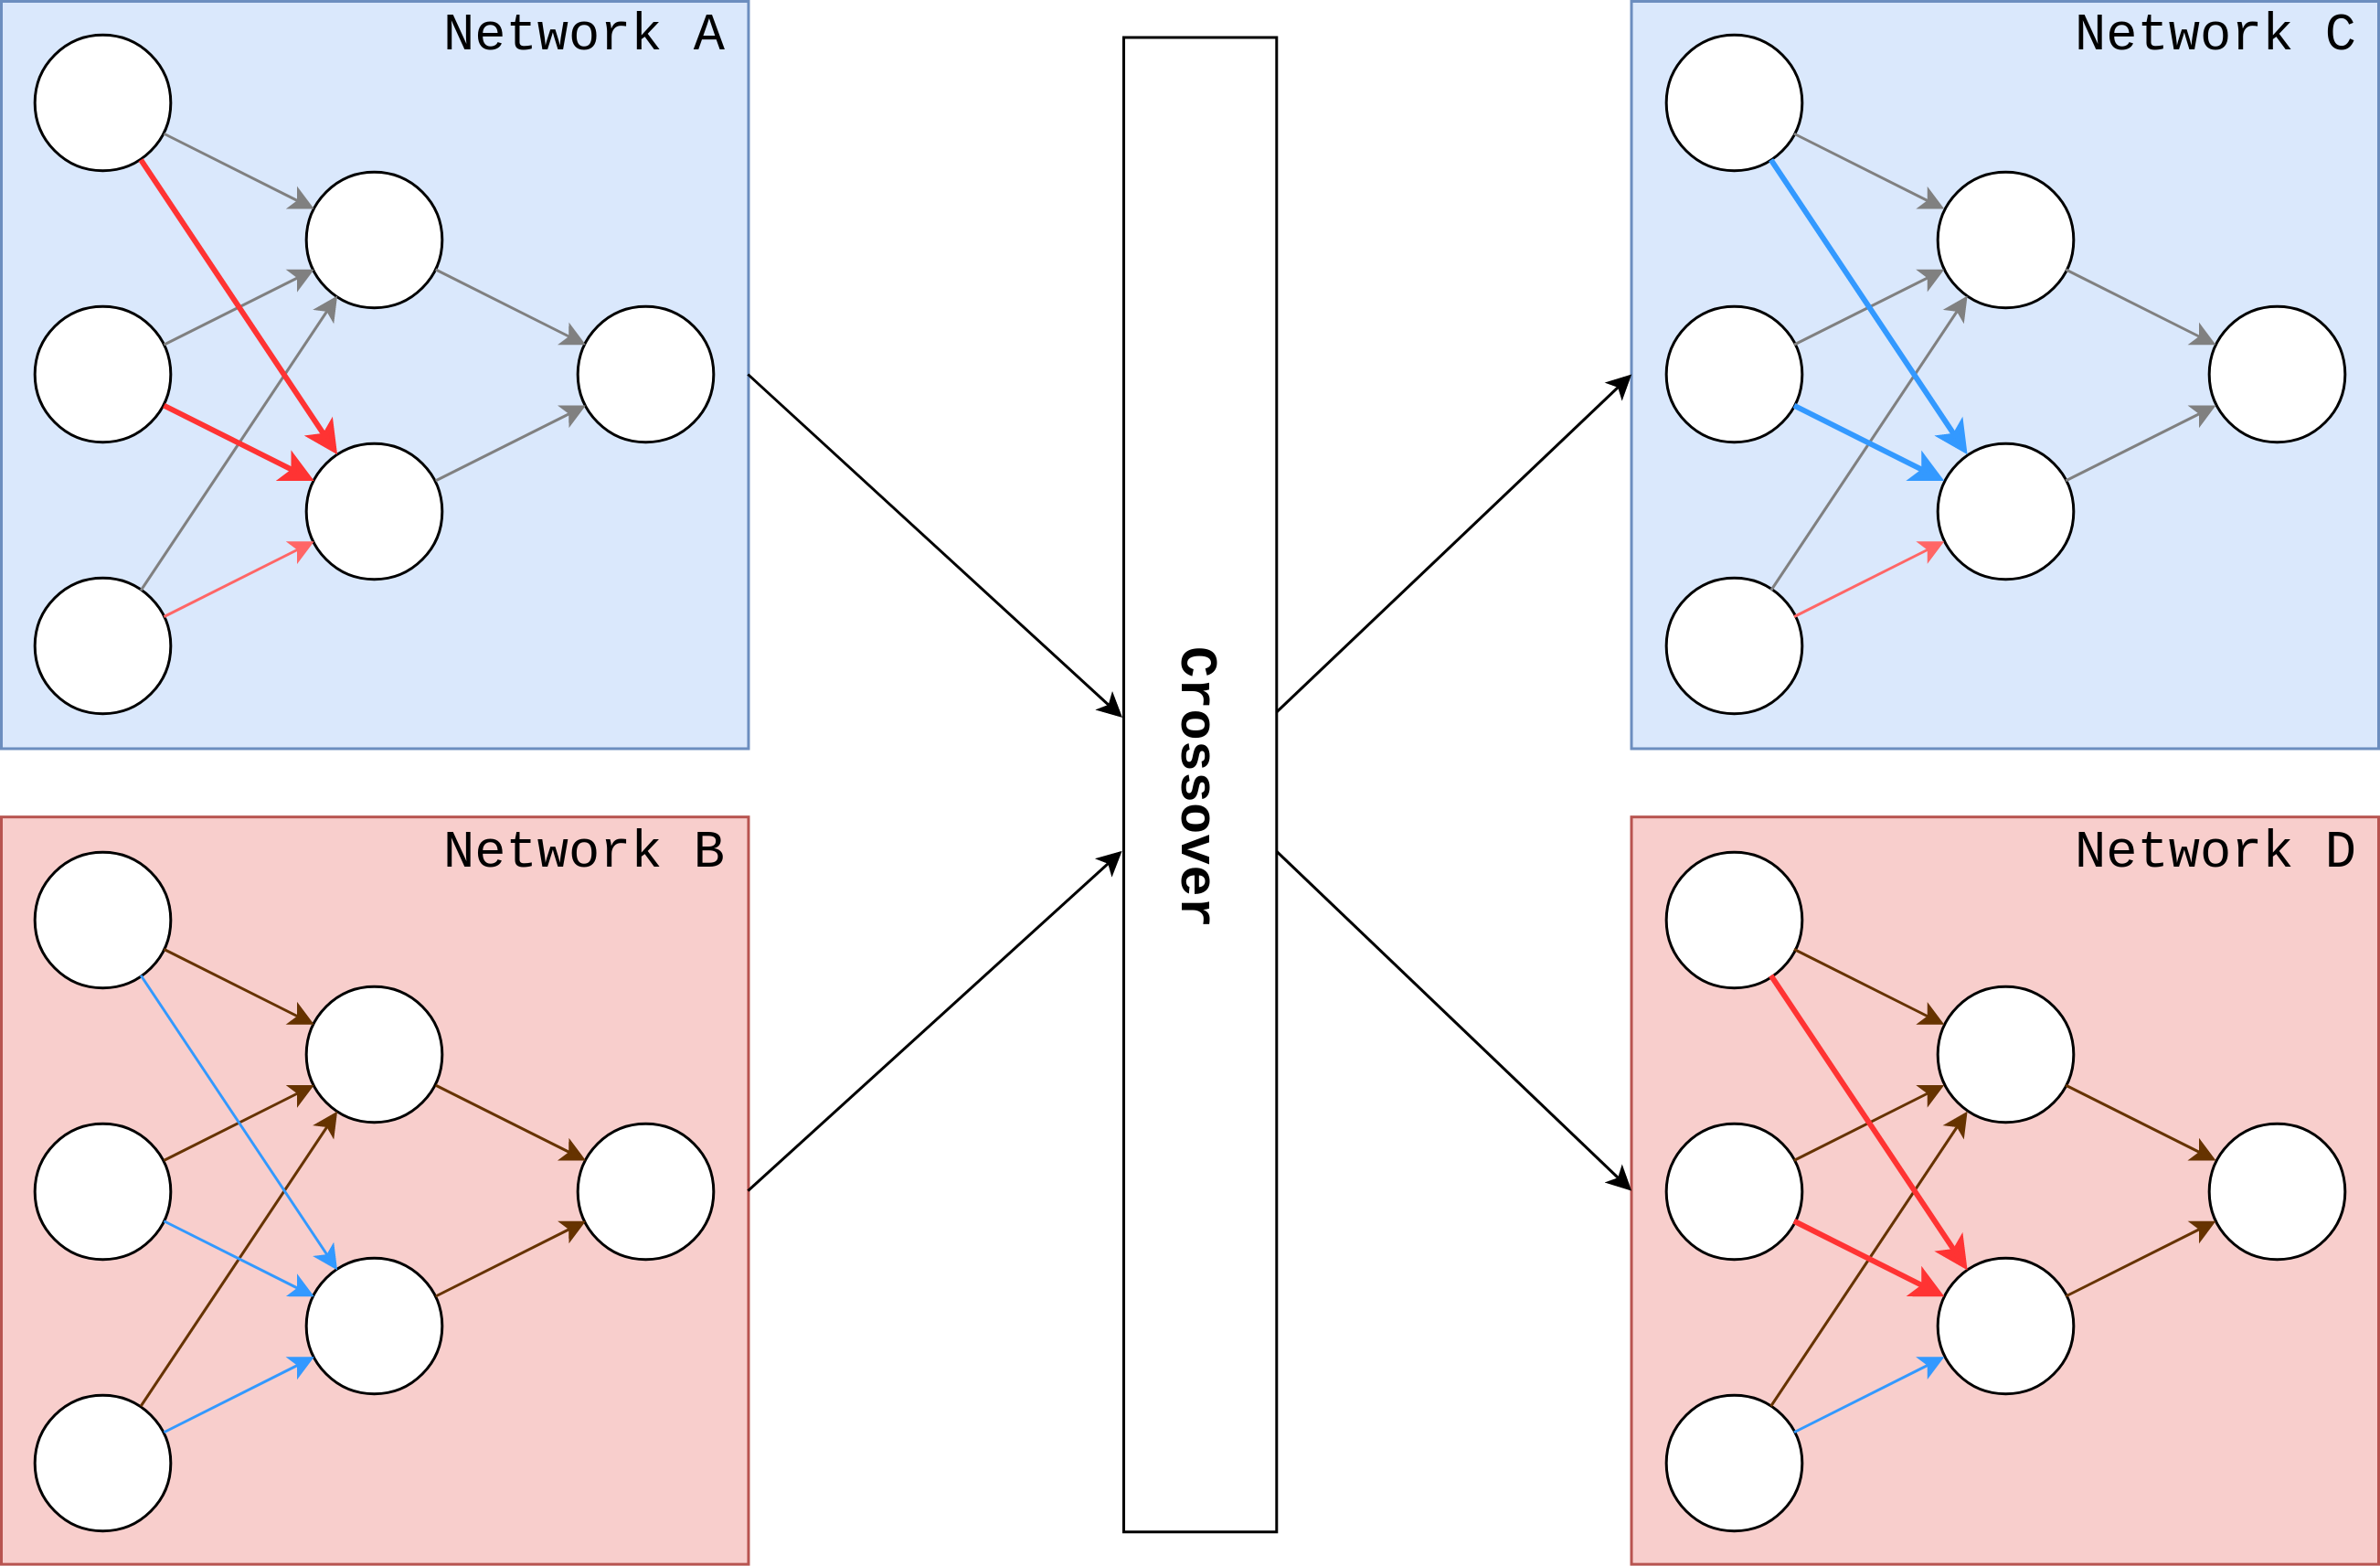
\includegraphics[width=90mm]{images/crossover.png}
                \caption{A diagram visualising the crossover process.\label{crossoverpic}}
            \end{figure}

            Another learning mechanism provided from the use of genetic algorithms is the use of crossovers. This combines the traits that build two parent agents to create children. In our scenario we use the weights and biases of the parent's neural networks.

            Two offsprings would be created from a pair of parents, with each offspring being the reciprocal crossover of each other. 
            % The weights of both parents (now each treated as a 1D array of coefficients), are divided contingent on the number of weights and biases for a given layer. Each layer should be treated separately to reduce the potential dependency on a purely randomly generated neural network. For each set of weights in a given layer, Algorithm \ref{crossover} describes the crossover process in pseudocode.
            A random node from the dominant parent is chosen. A dominant parent is the agent who gained more points in the tournament round than the other (who would be the submissive parent). If a dominant parent cannot be deduced it would be randomly chosen. 

            Once a random node is chosen, a subset of weights and biases that are fed to the chosen node are swapped with the submissive parents values at the same positions. As values in the weights can range from -1 to 1, dominant input weights are values that are greater than 0.75 or less than -0.75. Figure \ref{crossoverpic} shows this in more detail. In the diagram, Network A and B are parents, creating reciprocal offspring networks C and D. A is the dominant network, and A's node with the red inputs is chosen. The weights and biases of the red inputs are swapped with the values at the same position in network B. Network C is formed with Network B's dominant weights, with the rest being composed from A. Network D is the reciprocal, having Network A's dominant weights and the rest from B. A visualisation of the crossover process can be found in Figure \ref{crossoverpic}.

            The crossover should create a subtle modification to a neural network, by swapping a small subset of weights and biases at a time. Having a more dramatic crossover could potentially change the structure of the network flow, reducing its effectiveness. 
            
            % Talk about how this is not commonly used.

    \subsection{Testing}

        At the end of a given generation, we measure growth of performance by using the generation's champion. Presently the mean of means approach is used. When a new champion is generated, it is played against the previous 5 champions from earlier generations. 6 games are played for each previous champion, with 3 being as Black, and 3 being White. A mean score is calculated from those 6 games. The overall performance of the current champion is the mean of the 5 sets of games. A positive improvement is when the mean of means are greater than 0. Point Score for the champion games are measured by {1,0,-1} where a Win counts as 1 point, 0 for a draw, and -1 for a loss. The weights are scaled differently to the regular tournament in order to accurately portray the learning rate.
    
        \subsubsection*{Evaluation Method}
    
        The end player is used to create comparison games against its ancestors. This player is to be first tested against an agent who is choosing random moves to verify that the system is not playing arbitarily. Measurements from these games, alongside its champion scores be used as evidence to determine whether the agent is learning over time, is used to answer to answer the research question.
       
    % Issues
    \subsection{Setup and Issues}
        Initial runs will operate on a 1 and 2-ply load to determine the stability of the system on a linux (Ubuntu) machine containing a 4-core Intel i5 6600u processor with 12GB's of memory. Development and debugging will also occcur on this machine. Once testing has proven to be stable, the system would run on Durham's MIRA distributed system (Debian) with a 1,3 and 6-ply move depth. This machine utilises 4 Intel Xeon E7-8860 processors (Each CPU contains 16 physical cores running in 2.2Ghz, with hyperthreading). This comes to a total of 64 Cores, and 128 threads. MIRA also comes with 256GB of DDR3 memory. 
        
        To keep simulations running on MIRA, MOSH is used to maintain a consistent connection to MIRA. The end champion is then transferred to the initial machine in order to be played against by human input. Statistical evaluations and calculations are also calculated on MIRA to reduce computational time.
       
        Verifying that the moves are properly chosen was difficult and slow as games need to be played out first, with the quality assurance handled afterwards. The system was implemented first with the use of minimax search, but this cannot be used for the final measurements as the scalability of the decision making algorithm scales expoentially, as described prior.

        Interestingly, the machine used for training did not perform necessarily as effeciently. Although the system is built such that the games in the tournaments are "embarassingly parallel", the machine does not scale accordingly. Most of the computation is spent on calculating floating point matrix operations (Which represents the neural network evaluations.) Later research has shown that the use of hyperthreading does not necessarily show to scale the performance, even though more threads exist. \cite{leng_empirical_2002} This is due to the shared floating point arithmetic registers in the CPU, where two threads utilise the registers of one physical core. The use of GPU acceleration is not considered due to the lack of access. 
    
% TODO (WAIT FOR RESULTS)
\section{Results}
    %   Results:
    %   - Does it work?
    %   - Perhaps some measurable outcomes where appropriate.
    % this section presents the results of the solutions.  It should include information on experimental settings.  The results should demonstrate the claimed benefits/disadvantages of the proposed solutions.
    

    % This section should be between 2 to 3 pages in length.

    For the experiment, we create three different neuroevolutionary agents with seperate ply-depth: 1,3 and 6. Ply Depths 1 and 3 are run for 100 generations, and 6 is run for 200 generations to measure the overall potential of the system. For sections containing three charts, each chart represents the results of the agents playing at 1-ply, 3-ply, and 6-ply, respectively, in that order. Each simulation utilises a population of 15 agents.

    \subsection{Learning Rate}
    % chart of performance over time
    
    The learning rate is derived by comparing a generation's champions with its predecessor  champions from the previous five generations. For each older champion, six games are played, with the outcome of the current champion's performance scored and tallied up. An average of the six outcomes are calculated, representing the learning rate. We do not take the learning rate of the first 2 champions as this would not produce a sufficent comparison. This measurement is performed for every generation until the end of training. It is also the case that this does not influence the actual learning process of the system, but is used as one of the indicators of whether the system is learning in ability over time.
    
    \begin{figure}[!h]
        \centering
        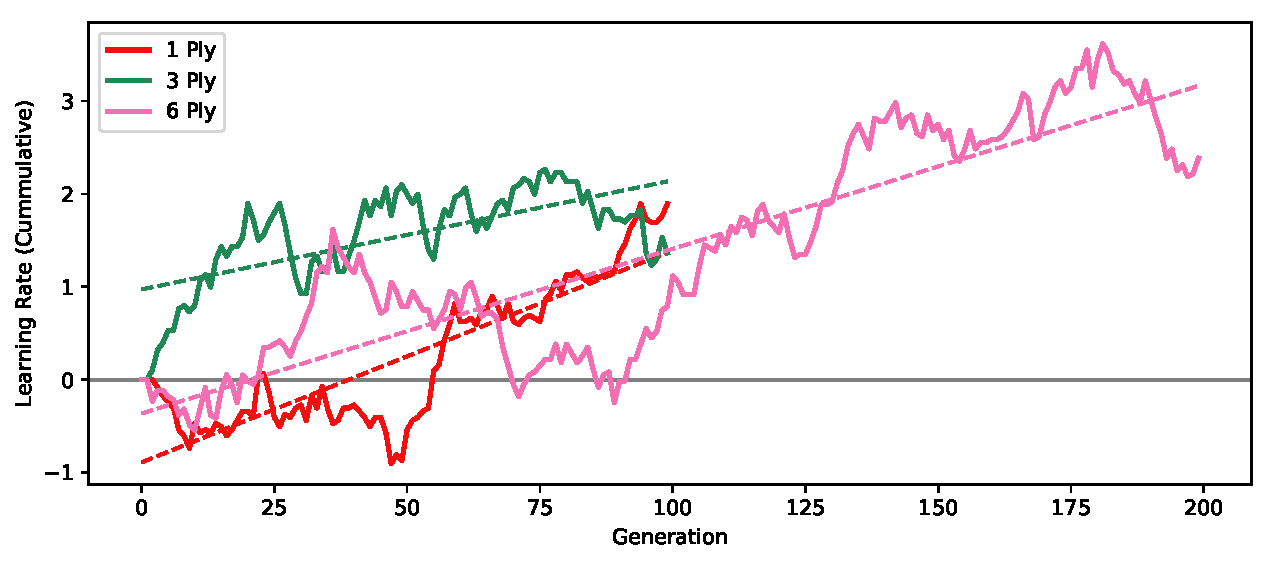
\includegraphics[width=160mm]{images/results/combined_cummulative.pdf}
        \caption{A chart showing the cummulative learning rate across the generations for the different ply depths.\label{cum_growth}}
    \end{figure}
    
    For all plys, we can see a cummulative growth such that returns are in the net positive as more generations are added. However, even with safe mutations, we can also see that the learning is very volatile. As the champion is chosen from a tournament, it may be related to the quality of the following generations having a lower ability to evaluate the board than it's parent generation. This could potentially be prevented by reusing the previous champion and restarting a particular generation if a loss can be seen. This could however tunnel the system towards a local maximum in terms of learning. Further measurements are taken to understand the reasoning of the potential troughs in learning. 
    
    \subsection{Performance}
    To measure the system performance at the end of training, the champion of the final generation is compared against a subset of their predecessors. For each precessor, the trained system plays 128 games (half as black and the other for white), and the number of wins, losses and draws are counted to produce the following statistics. For debugging purposes, all agents are also played against a random program to determine whether the system is evaluating moves properly. Fortunately, all agents successfully won every game.
    % compare the bots against a minimax agent
    % chart of previous champions
    \begin{figure}[!h]
        \centering
        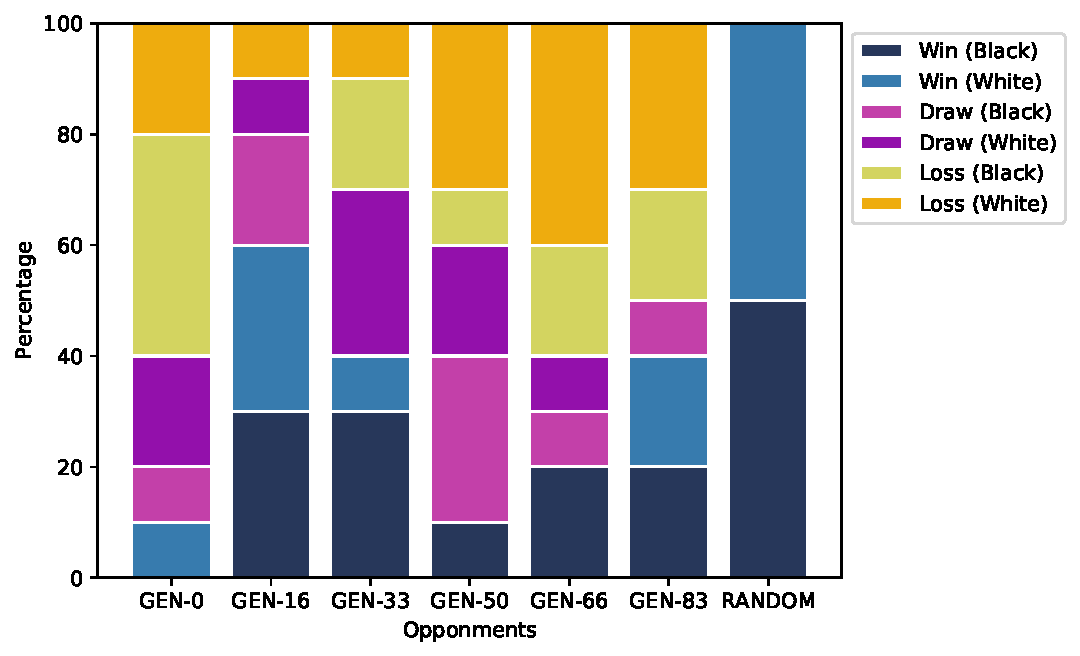
\includegraphics[width=53mm]{images/results/1ply/gm_net_stats.pdf}
        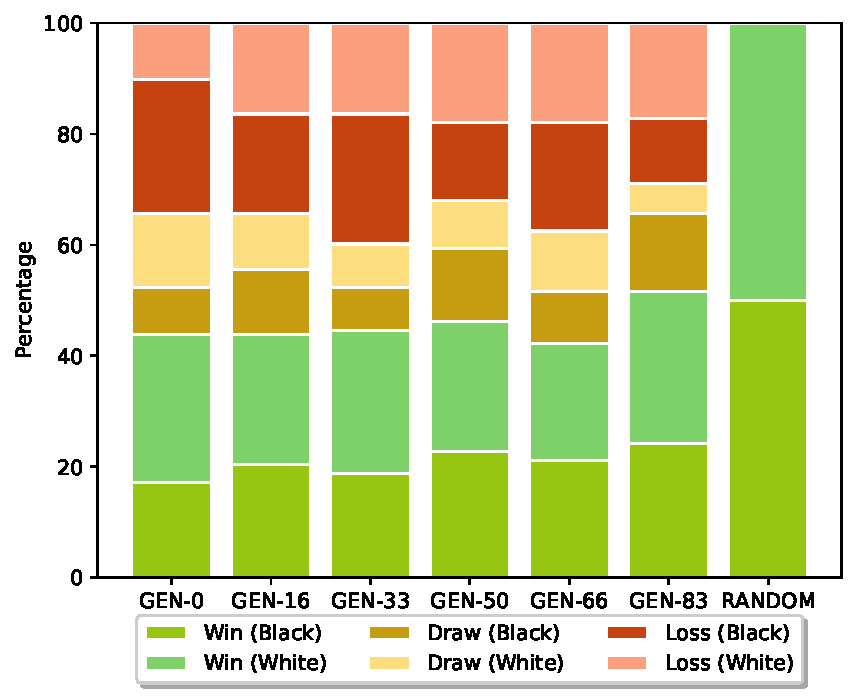
\includegraphics[width=53mm]{images/results/3ply/gm_net_stats.pdf}
        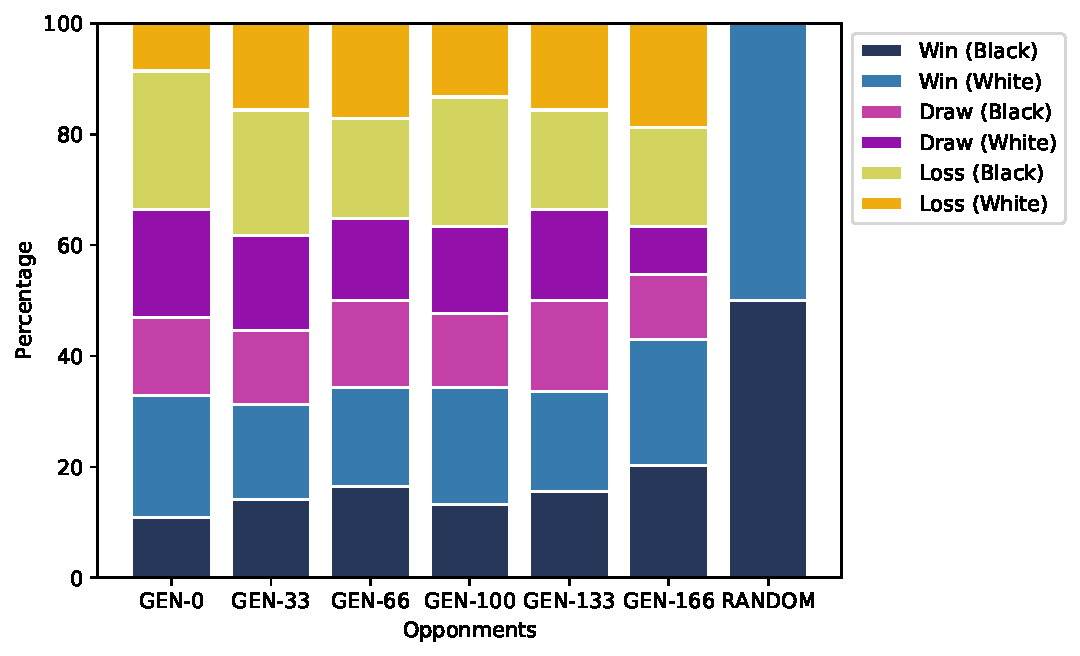
\includegraphics[width=53mm]{images/results/6ply/gm_net_stats.pdf}
        \caption{Charts showing the performance of the trained systems against their ancestral counterparts.\label{net_stats}}
    \end{figure}
    
    For the ply depth of 1, we can see an immediate net trend, with the end system beating earlier generations except for the first generation. This may make sense, as heuristic retention would be lost as the search depth is so low. This does however suggest that the system is worse off than playing with an initialised system (without training). For the higher ply depths (3,6) however, the agents manage to consistently maintain a higher chance of winning/drawing against their earlier counterparts. It is difficult to see a trend line. For the 6-ply, it is evident that there is an increase of draws caused against the earlier agents, which could be seen as an advantage.

    \subsection{Champion Distribution}
        The following charts shows the following distribution charts the champions of the generations. The intention behind this measurement is to determine whether champions are inherently chosen based on the influence of mutations, crossovers of simply elitism.  Measurements are taken such that the champion of each generation is looked at, and their genomic properties are collated to show a distribution of the chances of a particular agent being the champion. Note that while every offspring is mutated, some of the offsprings are created using genomic crossovers, described in section \ref{crossover_strategy}. 

        \begin{figure}[!h]
            \centering
            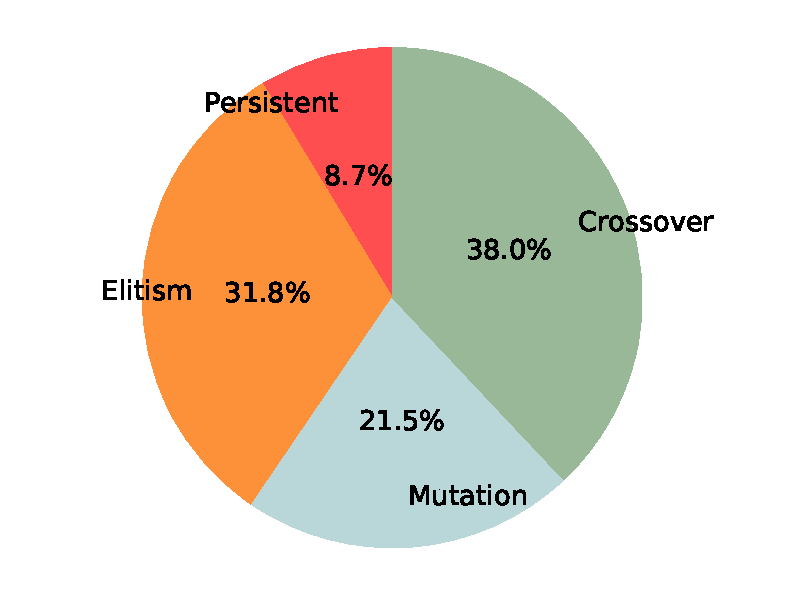
\includegraphics[width=53mm]{images/results/1ply/champ_gen_dist.pdf}
            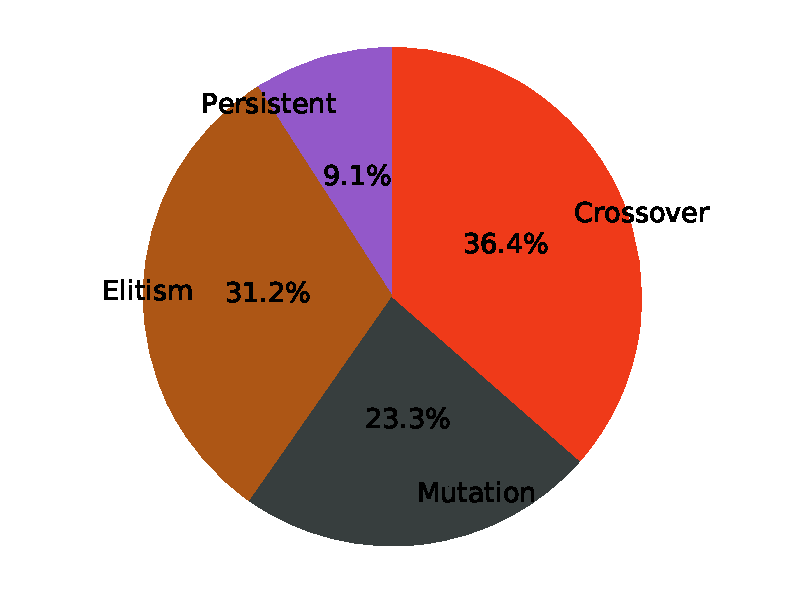
\includegraphics[width=53mm]{images/results/3ply/champ_gen_dist.pdf}
            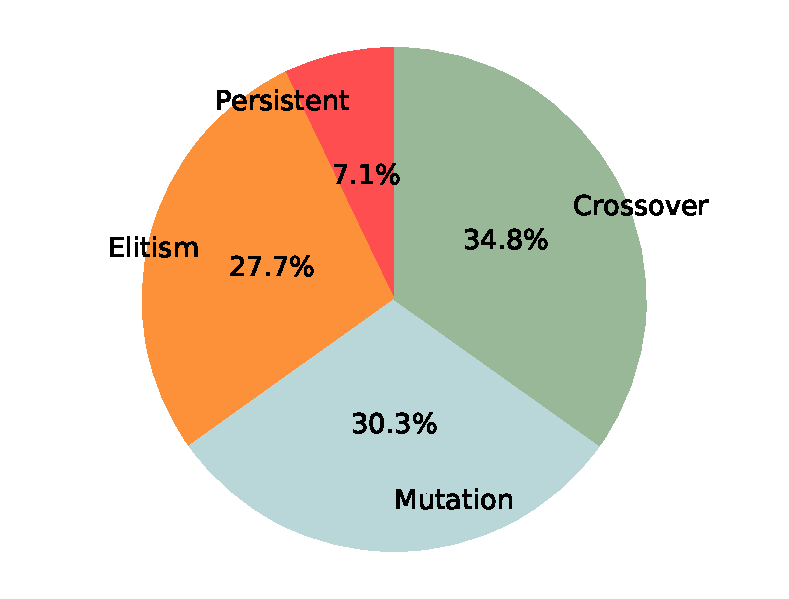
\includegraphics[width=53mm]{images/results/6ply/champ_gen_dist.pdf}
            \caption{Distributions of the different genomic identities across the tournament champions. \label{champ_gen_dist}}
        \end{figure}

        The influence of offsprings become more apparent for larger plys, with mutation and crossover appearing more frequently, coming at 66.1\% of the distribution. Interestingly, for ply depths 1 and 6, crossovers tend to be the most frequent occurence when it comes to producing champions at every generation. This suggests that crossover methods tend to produce better agents than their counterparts.

    \subsection{Influence of Inheritance Methods}
        Building on from the chart provided by Figure \ref{champ_gen_dist}, we look into the scores retrieved by the different genomic identities when they are compared against their earlier counterparts. This is to determine whether the use of genetic algorithms can overall improve the quality of neural networks. To measure this, we correlate the generation's champion with their score (the same measurement used to evaluate the learning rate in Figure \ref{cum_growth}) produced when measured against their predecessors. The results are shown in Figure \ref{champ_score_distribution}.

        \begin{figure}[!h]
            \centering
            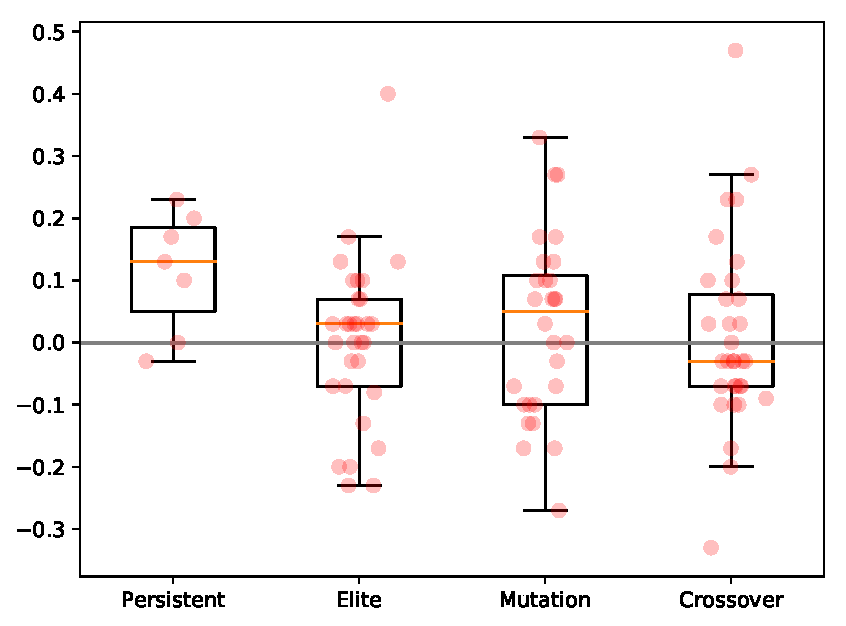
\includegraphics[width=53mm]{images/results/1ply/champ_score_distribution.pdf}
            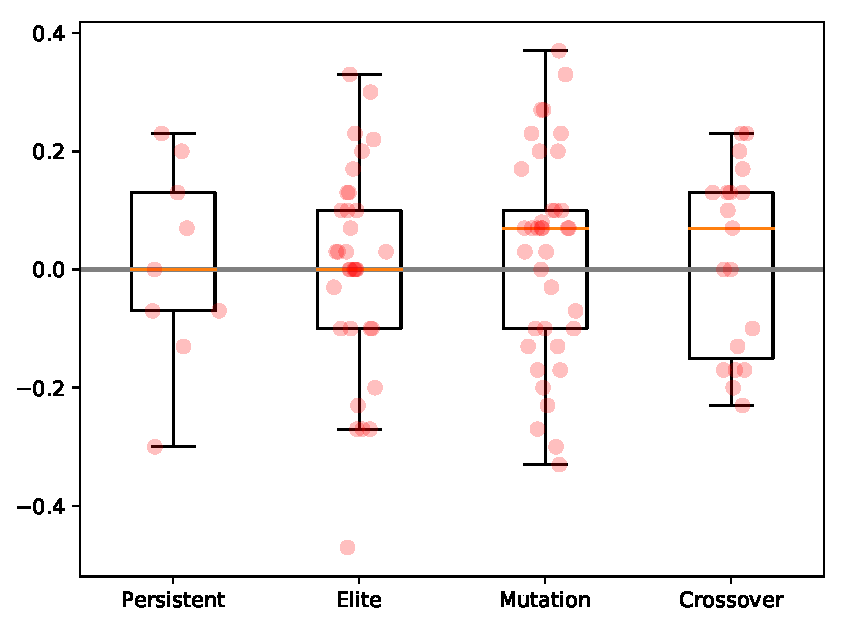
\includegraphics[width=53mm]{images/results/3ply/champ_score_distribution.pdf}
            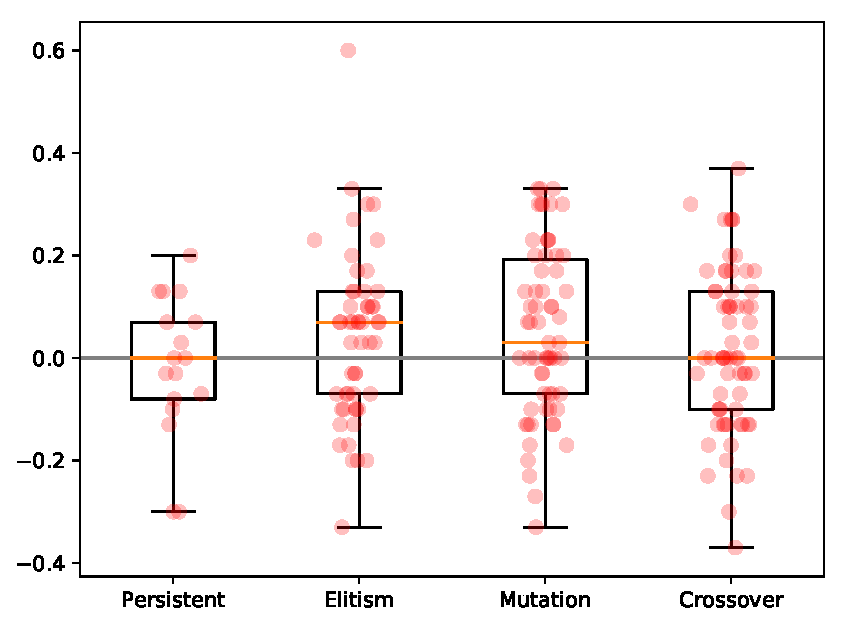
\includegraphics[width=53mm]{images/results/6ply/champ_score_distribution.pdf}
            \caption{Box-Plots of the different genomic identities and their distribution of scores. The yellow line in the box represents the mean score. \label{champ_score_distribution}}
        \end{figure}

        Interestingly, for the 3-ply, the crossover method is most likely to produce a growing system, producing the highest mean. However, across all of the ply depth agents, we can see that the use of mutation produces the best possible agents. For the higher 6-ply depth we can see that it did not significantly influence the learning rate of the system.

    \subsection{Other Observations}
        \subsubsection{Number of Moves}
            The number of moves is measured to verify that the system is producing realistic and quality moves over the training phase. The following charts show the distribution of moves for the games played over the generations, alongside the mean. The results are shown in Figure \ref{move_chart}:

            \begin{figure}[!h]
                \centering
                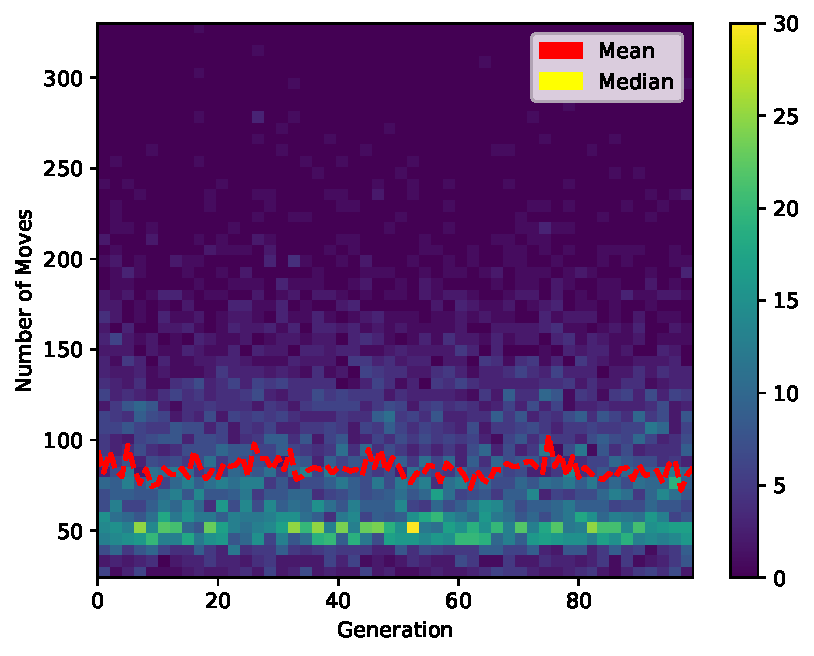
\includegraphics[width=53mm]{images/results/1ply/moves.pdf}
                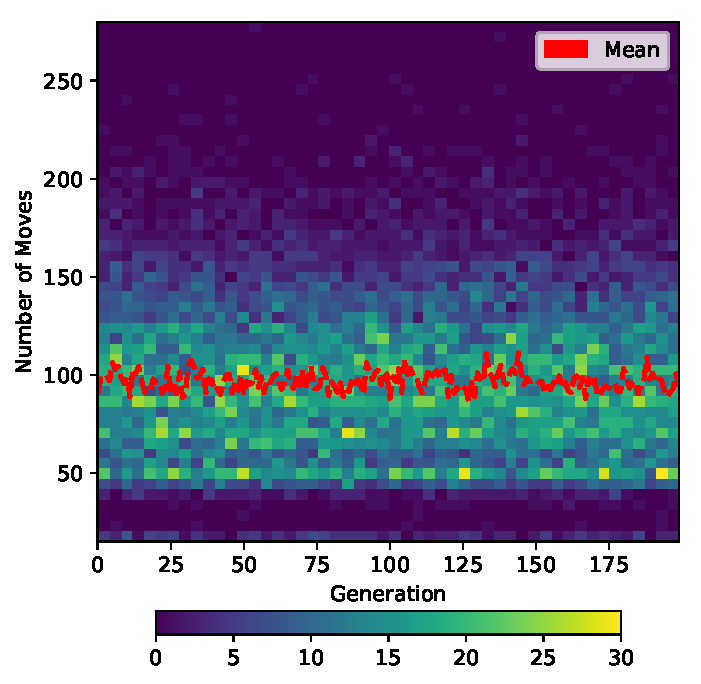
\includegraphics[width=53mm]{images/results/3ply/moves.pdf}
                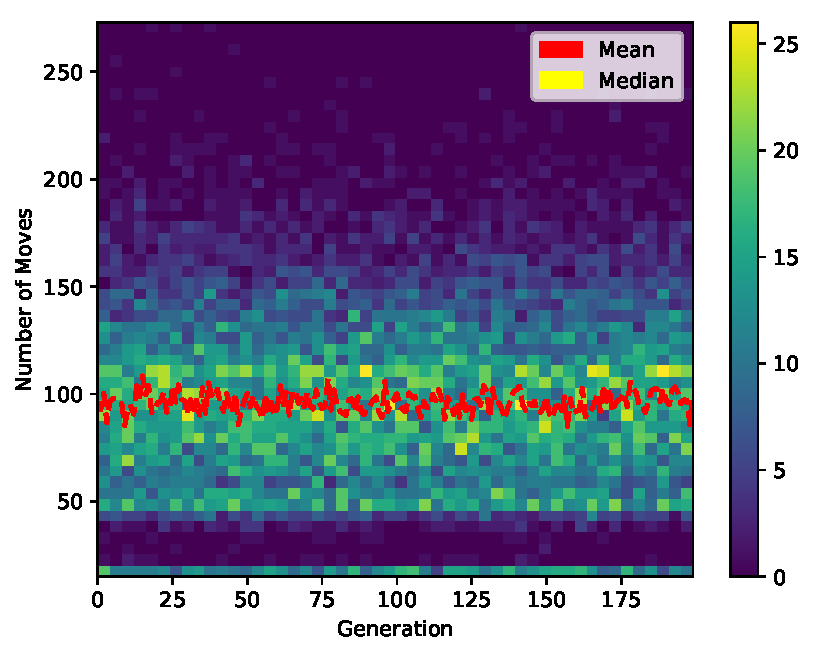
\includegraphics[width=53mm]{images/results/6ply/moves.pdf}
                \caption{2D Histograms representing the number of moves played in the games played in the generations. \label{move_chart}}
            \end{figure}

            % The number of moves is consistent throughout as the players are evaluating by projecting their own abilities to the opponment, leading to a fairly even distribution of moves across the generations. 

            For the 1-ply simulations, the average mean of moves is lower, but is counteracted by the much larger range of games that have a large number of moves. Understandably, the lower quartile for the 1-ply is lower than the others. This may be due to the level of precision, where it does not think further ahead enough to make better moves. This explanation applies inversely for the larger ply-depths, notably the 6-ply chart, where the level of precision is higher, leading to a tighter distribution of games having similar numbers of moves played.

            As the system is shown to play fairly consistently across the generations, this verifies that the system is choosing consistent decisions across the board. This confirms that the decision making algorithm is implemented precisely, reducing the number of unknowns for evaluation.

        \subsubsection{CPU Times}

            \begin{table}[]
            \centering
            \caption{Mean and Net running times of system training for the various depths.}
            \label{my-label}
            \begin{tabular}{ccccc}
                                        & 1-Ply                               & 3-Ply                                      & 6-Ply                                       &  \\ \cline{2-4}
            \multicolumn{1}{c|}{Mean} & \multicolumn{1}{r|}{0:04:24} & \multicolumn{1}{r|}{0:17:32}        & \multicolumn{1}{r|}{0:38:45}         &  \\ \cline{2-4}
            \multicolumn{1}{c|}{Net}  & \multicolumn{1}{r|}{7:21:25} & \multicolumn{1}{r|}{1 day, 5:14:41} & \multicolumn{1}{r|}{5 days, 9:12:25} &  \\ \cline{2-4}
                                        &                                     &                                            &                                             & 
            \end{tabular}
            \end{table}
            
            The system is shown to grow in running time linearly, as this is the cause of growing the search limit for MCTS in a linear fashion according to the ply-depth.

            \begin{figure}[!h]
                \centering
                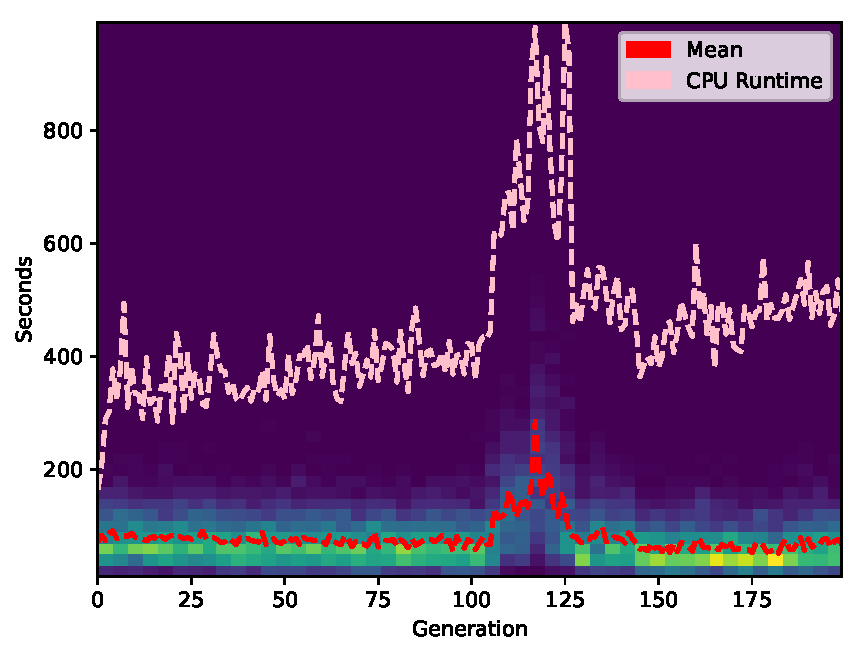
\includegraphics[width=53mm]{images/results/1ply/simulation_timings.pdf}
                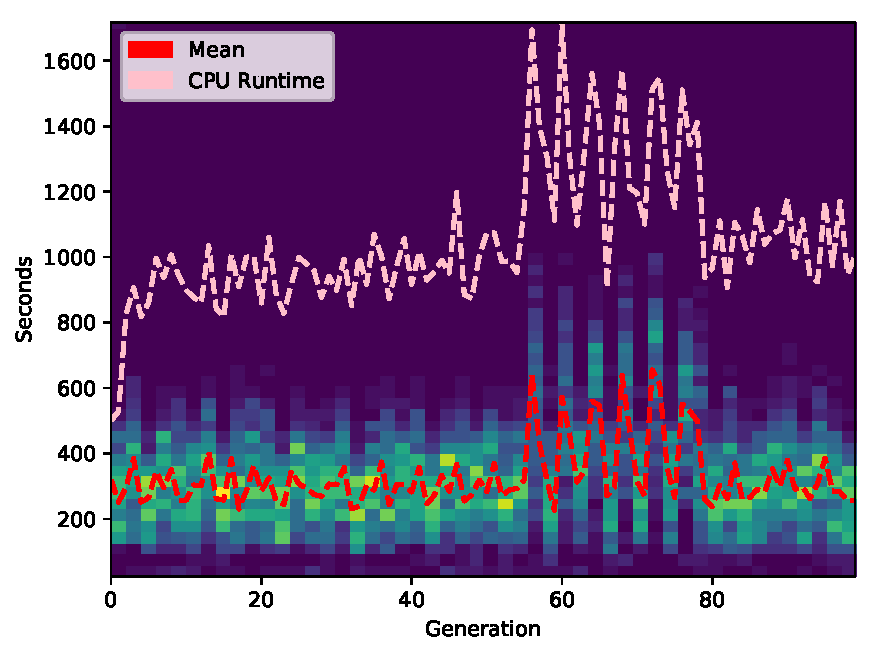
\includegraphics[width=53mm]{images/results/3ply/simulation_timings.pdf}
                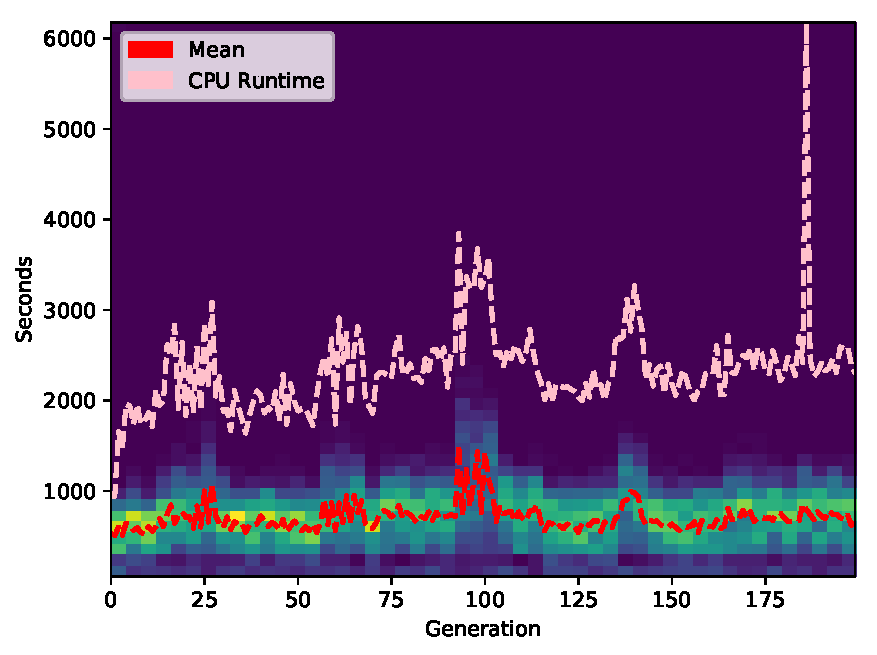
\includegraphics[width=53mm]{images/results/6ply/simulation_timings.pdf}
                \caption{2D Histograms of the average times spent on the games during the simulations. \label{chart_cpu_times}}
            \end{figure}

            The results suggest that the CPU time is very unstable, and is one of the downfalls of using a time-shared machine. The performance increase does not show to correlate with the learning rate. 

% TODO (WAIT FOR RESULTS)
\section{Evaluation}
    % Structure and content very project-dependent.
    % Follow the Design Report. Use the feedback.
    % Rule of thumb:
 
    %   Evaluation:
    %   - How well does it work?
    %   - Does it do what you wanted it to do?
    %   - How well did you do?
    %   - Did the plans pan out?

    We now reflect back to the original research question: "is it possible to create a performing draughts playing agent by the use of Genetic Algorithms and Neural Networks?".  We answer this through the examinations of the strengths and limitations of the system. 

    \subsection{Strengths}
    The statistics indicate that the system is indeed learning over time. This suggests that  neuroevolution is a viable method for programs with vast search spaces. While this is where both genetic algorithsm can shine. Although this is the case for Deep learning and evolutionary computation in general, the benefit of using genetic algorithms is that the fitness function can be any function, whereas for a neural network, its function needs to be translatable to some form of a differential sum of partial derivatives. 

    The system itself relies on a relatively simple learning heuristic that is open to domain specific adaptation. 
    Because the agents are essentially playing itself to learn over time, no training data is necessary for the program to evolve itself.

    embarrassingly parallel tournaments make it possible to reduce the overall system running time on the system.

    The use of crossovers, which differentiates genetic algorithms and its other evolutionary algorithms has shown to improve the quality of the players, especially the case in the 3-ply.

    \subsection{Limitations}
    The overall training rate is slow. Naturally slower learning rate than typical ventures as there is an immediate comparision to make against, and requires many more samples (often expoentially more) to get a weight of equivalent quality.
    The quality of the neuroevolutionary algorithm boils down to the quality of the fitness function, which in our case is the tournament method. Round-Robin is not necessarily the most efficent (from a number of games played perspective, and not necessarily parallelism) and does not eliminate cases where there is an ambiguous decision between the champions (which could be due to several players having an equal number of points). It also computes the most number of games. 
    - creating a high quality fitness function is difficult and its domain specific, or rather, there is no universal fitness function for all problems. This poses as a benefit and a weakness for the neuroevolutionary approach.
        - the fitness function defines the size of the search space and how easily a globally optimal solution can be derived.
        - using a best of champions approach is quite difficult!
        - reality rarely fits into good fitness functions
    The crossover mechanism is a hit and miss, and is shown to impede the learning rate for some of the longer ply-depths. This may be due to its disruptive nature, as heuristics are destroyed. As feared by findings by \cite{emmanouilidis_comparison_2000}, we can see the potential fears of the negative influence of the textbook crossover mechanism, where it has shown in the results to discourage learning.

    % The challenge with all GA work is finding the right fitness function. If you don't understand your domain well enough to define a good fitness function you're going to be wasting your time, and no amount of algorithmic and/or AI magic is going to help you.
    \subsection{Approach}
        The modularity of the system implementation was pivotal to debugging the system. The program itself is quite sizable, and it helps that individual tests can be conducted in most cases. It also helps that the order of the implementation helps.

        Measuring the learning rate is quite difficult and arbitary, and may best be compared to against systems that are classified to play at a particular level. 

        As most of the experiments are constrained by computational power and time, it may be best to re-evaluate this concept until either computational resources are more available, such as the use of GPU acceleration. The system should also be left to run for longer generations as presently the results do not show a notably strong correlation. The lack of computational resources also influenced the number of experimental testings that can be measured, such as the population size, the number of generations and the learning rate. 
        
        Another consideration for the project is to experiment with different crossover algorithms that utilise the temporal difference between inputs and outputs. There is an incredibly vast scope of future work that would extend the project. One interesting avenue is to consider using a safer method to produce mutation, exercising other contemporary methods in machine learning. It may also be the case that more time could be spent in examining references outside of computer science. In this particular example, the algorithms used are inspired by various biological and neuroscientific understandings. More research into this field may assist in finding more creative methods of solving some of the issues concerning genetic crossover mechanisms and mutation rates.

% TODO (WAIT FOR RESULTS)

\section{Conclusions}
    % This section summarises the main points of this paper.  Do not replicate the abstract as the conclusion.  A conclusion might elaborate on the importance of the work or suggest applications and extensions.  This section should be no more than 1 page in length.

    In terms of fufilling its objectives, the project was an overall success. A system was implemented using evolutionary methods and it successfully plays checkers in a manner in which it can learn from over time. To the extent of its growth remains suspect however. Efforts to measure the learning rate is one of the non-trivial challenges that makes neuroevolution a particular field of interest, as it is inherent that it can tackle problems in a somewhat novel manner.
    
    The main findings of this project is as follows:
    \begin{enumerate}
    \item It is evidently possible to create a checkers playing agent that learns to play itself, with little human intervention.
    % - some of the the work is 
    \item  neuroevolution is relatively inefficent compared to their gradient based counterparts. This however forseen due to the heavy dependency of entropy disguised as learning.
    \item  The fitness function can be anything, but it is important to derive a high quality fitness function.
    \item The quality of crossovers can be a deciding factor in how the agents learn to play over time.
    \end{enumerate}

    The major implication is that it is a possible contender for tasks that require unsupervised learning, and that the fitness function cannot be trivially decomposed into set of derivatives that allow regular derivative based learning to shine.
    
    Provided a high quality fitness function can be designed, the applications of neuroevolution expand beyond its applications in zero-sum games. Neuroevolution in general is useful based on its ability to solve problems without the use of training data, and generating evolving content over time. When applied in a successful manner, its applications can go towards the  understanding of biological neural networks and the evolution of intelligence itself.

\bibliography{zotero}

\end{document}
